\section{CONTEO DE ESPECTROS SERIALES}\label{ch:espectros}
	\subsection{Espectros de las funciones \{I, T, R\}}
		\label{espec}
		Es interesante conocer el n\'umero de espectros seriales distintos que un compositor puede escoger. Al fin y al cabo, es irrelevante qu\'e serie se escoge como la original dentro de su espectro serial, ya que produce el mismo material compositivo que cualquiera de su mismo espectro.
		
		Para calcular el n\'umero de espectros seriales se redefinir\'an las funciones transformativas para una longitud serial arbitraria, $n$, que ser\'a mayor que 2. Para $n=0,\ 1$ y 2 se realizar\'a el c\'alculo en el apartado \ref{monodi}. 
	
		Adem\'as, como las transposiciones siempre son distintas entre s\'i, siempre pertenecen al mismo espectro. Se tomar\'an a partir de ahora todas ellas como equivalentes, de manera que solo se necesita hacer el c\'alculo para $\{I,\ R\}$.
		
		Al calcular con permutaciones se trabajar\'a m\'odulo $n$. La retrogradaci\'on sigue siendo $R(\sigma(m))=\sigma(-1-m)$. La inversi\'on ser\'a $I(\sigma(m))=-\sigma(m)$, omitiendo la transposici\'on habitual, ya que se toman las series transpuestas como equivalentes. De esta forma $-\sigma(m)+2\sigma(0)\equiv-\sigma(m)$. La retrogradaci\'on invertida es, por tanto, la composici\'on de ambas: $RI(\sigma(m))={I}\circ{R}(\sigma(m))={I}\left({R}(\sigma(m))\right)=-\sigma(-1-m)$.			
		
		La retrogradaci\'on, la inversi\'on y la composici\'on de ambas cumplen que al aplicarlas dos veces se vuelve a la serie original. En teor\'ia de grupos se dice que tienen \textit{orden 2}. Entonces $\{Id,\ I,\ R,\ IR\}$ forma el ya mencionado grupo de Klein ($\Xi$), donde $RI$ $\equiv$ $IR$, ya que estamos tomando las series transpuestas como equivalentes. 
		
		En general, un grupo de Klein es el formado por cuatro elementos donde cada elemento es inverso de s\'i mismo. El grupo de Klein, llamado as\'i en honor al matem\'atico alem\'an Felix Klein, es el grupo $\mathbb{Z}/(2)\times\mathbb{Z}/(2)$, producto directo de dos grupos c\'iclicos de orden 2.
		
		Por el lema de Burnside:
		\[\#\mbox{Espectros}=\frac{1}{|\mathbb{Z}/(2)\times\mathbb{Z}/(2)|}\sum_{\sigma\in{S}_n}|{Stab}(\sigma)|=\frac{1}{4}\sum_{\sigma\in{S}_n}|{Stab}(\sigma)|\]
		
		Es decir, se deben calcular para cada posible serie $\sigma\in{S}_n$ cu\'antas funciones transformativas lo dejan igual o equivalente bajo transposici\'on.
		
		Como los estabilizadores son subgrupos, por el teorema de Lagrange su tama\~no debe ser divisor del tama\~no del grupo total. Entonces se pueden agrupar los estabilizadores por sus tama\~nos: 1, 2 o 4, y as\'i calcular $\sum|{Stab}(\sigma)|$ agrupando todas las permutaciones con igual tama\~no de estabilizador. Si $\#\sigma_i$ es el n\'umero de permutaciones cuyos estabilizadores tienen tama\~no $i$:		
		\[\sum_{\sigma\in{S}_n}|{Stab}(\sigma)|=1\cdot(\#\sigma_1)+2\cdot(\#\sigma_2)+4\cdot(\#\sigma_4)\]
	
		Primero, se ha de ver que una permutaci\'on nunca va a ser igual ni equivalente mediante transposiciones a su inversa.\label{inversano}
			\begin{align*}
			-\sigma(m)&\equiv\sigma(m)\Longleftrightarrow\\
			0&\equiv2\sigma(m)\Longleftrightarrow\\
			n&\equiv2\sigma(m)\Longleftrightarrow\\
			\frac{n}{2}&\equiv\sigma(m)
			\end{align*}
		
		As\'i, $\sigma(m)$ ser\'ia constante para todo $m\in \mathbb{Z} / (n)$, lo cual es imposible. Esto implica que ninguna permutaci\'on va a tener a $I$ en su estabilizador, por lo que $\#\sigma_4=0$. Queda entonces calcular cu\'antas permutaciones son equivalentes a su retrogradaci\'on y cu\'antas a su retrogradaci\'on inversa. La suma de ambas dar\'a $\#\sigma_2$.
	
	\subsubsection[Elementos estables mediante $R$]{Elementos estables mediante $\bm{R}$}
		Las permutaciones que coinciden con alguna transposici\'on de su retrogradaci\'on cumplen, para $\gamma$ constante:
		
		\hspace*{8.5\bigskipamount} $\gamma+\sigma(m) = {R}(m) = \sigma(-1-m)$
		
		Aplic\'andolo a $(-1-m)$:
		$\gamma+\sigma(-1-m) = \sigma(m)$
		
		De ambas ecuaciones: $\quad\gamma=\sigma(-1-m)-\sigma(m)=\sigma(m)-\sigma(-1-m)$
		
		$2\sigma(m)\equiv2\sigma(-1-m)\implies2\sigma(m)-2\sigma(-1-m)\equiv0$
		
		$2\sigma(m)-2\sigma(-1-m)=n \implies \sigma(m)-\sigma(-1-m)=\frac{n}{2}$
		
		Entonces $n$ debe ser par. Cuando $n$ es impar este tipo de permutaciones no existe. Adem\'as, cumplen que sus elementos sim\'etricos se distancian entre s\'i un intervalo de $\frac{n}{2}$ unidades: son series con simetr\'ia par.
		\[\gamma=\sigma(m)-\sigma(-1-m)=\frac{n}{2}\]
		
		En una serie de longitud $n$, existen $\frac{n}{2}$ intervalos que miden $\frac{n}{2}$. Como no importa por cu\'al de ellos comience la serie, ya que las transportaciones son equivalentes, se fija el primero de los intervalos. Quedan los otros $\frac{n}{2}-1$ intervalos por escoger, as\'i que el n\'umero de series con simetr\'ia par cuenta las permutaciones de $\frac{n}{2}-1$ intervalos y las dos posibles posiciones de cada intervalo \textemdash creciente y decreciente~\cite{reiner}\textemdash. Por ello, el n\'umero de series con simetr\'ia par es de:
		
		\[2! \cdot \left(\frac{n}{2}-1\right)! = 2\left(\frac{n-2}{2}\right)!=(n-2)(n-4)\ldots=(n-2)!!\]
		
		Por definici\'on, si $n$ es par $n!!=n(n-2)(n-4)\ldots4\cdot2$ y si $n$ es impar $n!!=n(n-2)(n-4)\ldots3\cdot1$.

	\subsubsection[Elementos estables mediante $RI$]{Elementos estables mediante $\bm{RI}$}
		Las permutaciones que coinciden con alguna transposici\'on de su retrogradaci\'on inversa cumplen, para un $\gamma$ constante:
		\[\sigma(m)={RI}(\sigma(m))+\gamma=-\sigma(-1-m)+\gamma\]
		\[\gamma=\sigma(m)+\sigma(-1-m)\]
		
		Sus elementos sim\'etricos suman una cantidad constante: son series con simetr\'ia impar. Tal y como se ha hecho en el apartado anterior, se puede fijar una de las notas, ya que las transportaciones son equivalentes. Si $n$ es impar, la nota central es $\sigma(\frac{n-1}{2})$, que es igual a $\sigma(-1-\frac{n-1}{2})$. Por tanto, $\gamma=2\cdot\sigma(\frac{n-1}{2})$. Si se escoge esta nota para ser fijada a 0, entonces $\gamma=2\cdot0=0$. Es decir, $\gamma$ puede ser fijada a 0 sin p\'erdida de generalidad.
		
		Para el resto de notas, $\sigma(m)=-\sigma(-1-m)$. Ya escogida la nota central, permite $n-1$ posibilidades para $\sigma(0)$. Ya escogidas la nota central, la primera y su sim\'etrica, permiten $n-3$ posibilidades para $\sigma(1)$, y as\'i sucesivamente hasta llegar a la nota anterior a la central, que es $\frac{n-3}{2}$. Por ello, para $n$ impar, el n\'umero de series con simetr\'ia impar es de:	
		\[(n-1)(n-3)\ldots(n-2\cdot\frac{n-5}{2}-1)(n-2\cdot\frac{n-3}{2}-1)=\]
		\[=(n-1)(n-3)\ldots(n-(n-5)-1)(n-(n-3)-1)=\]
		\[=(n-1)(n-3)\ldots4\cdot2=(n-1)!!\]
		
		Si $n$ es par, $\sigma(m)\neq\sigma(-1-m)\ \forall m\in \mathbb{Z} / (n)$, ya que no hay elemento central. Sea ahora $\gamma=2k$ un n\'umero par. Como $2k\leq n$ y las permutaciones son suprayectivas, para alg\'un $m$ se cumple que $\sigma(m)=k$. Se tiene entonces $k+\sigma(-1-m)=2k\implies\sigma(-1-m)=k=\sigma(m)$. Como esto es una contradicci\'on, $\gamma$ debe ser impar.
		
		Fijando, por ejemplo, $\sigma(0)=0$, se tienen $\frac{n}{2}$ posibilidades para $\sigma(-1-m)$, es decir, solamente las posibilidades para las que $\gamma$ es impar. Para $\sigma(1)$ hay $(n-2)$ posibilidades, y ahora su sim\'etrico ya viene determinado por el $\gamma$ escogido. Para $\sigma(2)$ hay $(n-4)$, y as\'i sucesivamente~\cite{reiner}. Por tanto, para $n$ par, el n\'umero de series con simetr\'ia impar es de: 
		\[\frac{n}{2}\cdot(n-2)(n-4)\ldots(n-2\cdot\frac{n-4}{2})(n-2\cdot\frac{n-2}{2})=\]
		\[=\frac{n}{2}\cdot(n-2)(n-4)\ldots(n-(n-4))(n-(n-2))=\]
		\[=\frac{n}{2}\cdot(n-2)(n-4)\ldots4\cdot2=\frac{n}{2}\cdot(n-2)!!\]
			
	\subsubsection*{Suma completa}
		Como ya se ha podido observar, el n\'umero de espectros seriales var\'ia seg\'un la paridad de la longitud de las series.		
		\def\arraystretch{1.5}
		\[\begin{array}{c|c|c|c|c}
		&\{Id,\ I\}&\{Id,\ R\}&\{Id,\ RI\}&\#\sigma_2\\\hline
		n\mbox{ impar}&0&0&(n-1)!!&(n-1)!!\\\hline
		n\mbox{ par}&0&(n-2)!!&\frac{n}{2}\cdot(n-2)!!&\frac{1}{2}(n+2)(n-2)!!\\
		\end{array}\]
		\def\arraystretch{1}
		
		Una vez se tiene $\#\sigma_2$, solo falta calcular $\#\sigma_1$. Como las permutaciones contadas $\#\sigma$ son todas las de ${S}_n$ exceptuando las transportaciones, $\#\sigma=\frac{\#\mbox{S}_n}{n}=\frac{n!}{n}=(n-1)!$. Por otro lado, $\#\sigma_1 +\#\sigma_2=\#\sigma$. Entonces $\#\sigma_1=(n-1)!-\#\sigma_2$.
		
		Recuperando la f\'ormula del apartado \ref{espec}:
		
		\[\#\mbox{Espectros}=
		\frac{1}{4}\left(\#\sigma_1+2\cdot(\#\sigma_2)\right)=
		\frac{(n-1)!+\#\sigma_2}{4}\]
		
		Para $n$ impar:
		\[\frac{(n-1)!+(n-1)!!}{4}=\frac{(n-1)!!\cdot\left((n-2)!!+1\right)}{4}\]
		
		Para $n$ par:
		\[\frac{(n-1)!+\left(\frac{1}{2}(n+2)(n-2)!!\right)}{4}=\frac{2(n-1)!+(n+2)(n-2)!!}{8}\]
		
		Para $n=12$, es decir, para el dodecafonismo, la \'ultima f\'ormula proporciona el dato de 9985920 espectros seriales a escoger por el compositor.
		
		Como ejemplo perteneciente al serialismo integral, podemos numerar las din\'amicas del 0 al 6:
		\[\{ppp,\ pp,\ p,\ m\!f,\ f,\ f\!\!f,\ f\!\!f\!\!f\} \equiv \{0,\ 1,\ 2,\ 3,\ 4,\ 5,\ 6\} = \mathbb{Z} / (7)\]
		
		As\'i, con la f\'ormula para $n$ impar, se obtiene que hay 192 espectros seriales con series de longitud 7.
	
	
	\subsection[Espectros del grupo $D_n\times D_n$]{Espectros del grupo $\bm{D_n\times D_n}$}
	
		Este apartado es una explicaci\'on detallada del art\'iculo \cite{polygons}. La secuencia de n\'umeros dada por las f\'ormulas que obtendremos se encuentra en la OEIS: \url{https://oeis.org/A000940}.
	
		\begin{figure}[h]
			\begin{center}
			\ddiagram[no numbers, no arrow]{4,5,7,1,6,3,8,2,11,0,9,10}
			\end{center}
		\end{figure}
		Ahora calcularemos los espectros formados mediante todas las transformaciones del grupo generado por $\{S,\ T,\ V,\ C\}$; es decir, por ${D}_{n}\times {D}_{n}$. Volviendo a la representaci\'on mediante diagramas de reloj, el problema es equivalente a averiguar cu\'antos diagramas distintos, sin n\'umeros ni flechas, se pueden dibujar. La flecha indica lo transformado por $V$ y $C$, mientras que los n\'umeros indican lo transformado por $S$ y $T$. Un diagrama sin estos dos elementos representa entonces todo un espectro serial. ¿Cu\'antos diagramas esencialmente distintos hay? De nuevo, por el lema de Burnside:
		\[\#\mbox{Espectros}=\frac{1}{|{D}_{n}\times{D}_{n}|}\sum_{\sigma\in{S}_n}|{Stab}(\sigma)|=\frac{1}{2n\cdot2n}\sum_{\sigma\in{S}_n}|{Stab}(\sigma)|\]
		
		En vez de expresar el sumatorio como ``para cada $\sigma$, el n\'umero de $\Psi$ que fijan $\sigma$'', se puede expresar como ``para cada $\Psi$, el n\'umero de $\sigma$ fijados por $\Psi$''. La f\'ormula queda de esta manera:
		
		\[\#\mbox{Espectros}=\frac{1}{4n^2}\sum_{\Psi\in{D}_{n}\times{D}_{n}}{Fij}(\Psi)\] 
		
		Ahora hay que averiguar para cada elemento de ${D}_{n}\times{D}_{n}$ cu\'antas series estabiliza. Por ejemplo, trivialmente no hay permutaciones estables mediante $C$ y $V$ solamente.
		
		
		\subsubsection[Elementos estables mediante $T$]{Elementos estables mediante $\bm{T}$}
		
		Los elementos estables mediante $T^{k}$ son a los que, tras aplicar una rotaci\'on de $\uptheta_{k}=\frac{2\pi k}{n}$, para $1\leq k\leq n$, quedan igual. Por tanto, los sumandos que aportan a la suma total son $\sum\limits_{k=1}^{n}{Fij}(\uptheta_{k})$.
		
		Por otro lado, si $1\leq p,q\leq n$ y $gcd(p,n)=gcd(q,n)$ entonces ${Fij}(\uptheta_p)={Fij}(\uptheta_q)$, ya que por el lema de B\'ezout lo que genera la rotaci\'on $\uptheta_p$ es igual a lo que genera la rotaci\'on $\uptheta_{{gcd}(p,n)}$. Esto permite que se puedan agrupar los sumandos con igual m\'aximo com\'un divisor con respecto a $n$. Es decir, $\sum\limits_{k=1}^{n}{Fij}(\uptheta_{k})=\sum\limits_{d|n}\left(\mathcal{C}\cdot{Fij}(\uptheta_d)\right)$, con $d$ divisor de $n$.
		Por ejemplo, si $n=6$:
		\begin{align*}
			&{Fij}(\uptheta_{1})+{Fij}(\uptheta_{2})+{Fij}(\uptheta_{3})+{Fij}(\uptheta_{4})+{Fij}(\uptheta_{5})+{Fij}(\uptheta_{6})=\\
			&{Fij}(\uptheta_{1})+{Fij}(\uptheta_{2})+{Fij}(\uptheta_{3})+{Fij}(\uptheta_{2})+{Fij}(\uptheta_{1})+{Fij}(\uptheta_{6})=\\
			&2\cdot{Fij}(\uptheta_{1})+2\cdot{Fij}(\uptheta_{2})+1\cdot{Fij}(\uptheta_{3})+1\cdot{Fij}(\uptheta_{6})
		\end{align*}
		
		
		Ahora queremos encontrar el coeficiente $\mathcal{C}$ de ${Fij}(\uptheta_d)$, es decir, el n\'umero de $k\leq n$ con igual m\'aximo com\'un divisor $d$. Pero que $k\leq n$ y $gcd(k,n)=d$ es equivalente a que $ \frac{k}{d}\leq\frac{n}{d}$ y $gcd\left(\frac{k}{d},\frac{n}{d}\right)=1$. Por tanto, el n\'umero de $k$ con m\'aximo comun divisor $d$ es $\varphi\left(\frac{n}{d}\right)$. La funci\'on $\varphi(x)$ se llama la funci\'on \textit{phi} de Euler, y muestra precisamente la cantidad de n\'umeros menores que \'el y coprimos con \'el. Entonces $\sum\limits_{{k}=1}^{n}{Fij}(\uptheta_{{k}})=\sum\limits_{d|n}\left(\varphi(\frac{n}{d})\cdot{Fij}(\uptheta_d)\right)$.
		
		Para calcular ${Fij}(\uptheta_d)$ hay que analizar c\'omo se construyen los diagramas invariantes respecto a una rotaci\'on. Estos diagramas deben tener varios \textit{ciclos} iguales entre s\'i \textemdash para que queden invariantes al rotarlos\textemdash~pero cada uno desde un punto distinto: desde cada m\'ultiplo de $d$. El n\'umero de ciclos es, por tanto, $\frac{n}{d}$.
		
		Al construir uno de estos diagramas, se escoge la primera nota entre las $n$. Despu\'es se escoge la segunda, pero no se pueden escoger los v\'ertices m\'ultiplos de $d$ (de los que hay $\frac{n}{d}$), ya que van a ser el comienzo de los sucesivos ciclos. Hay entonces $n-\frac{n}{d}$ posibilidades. Despu\'es se escoge la tercera, pero sin escoger los m\'ultiplos de $d$ ni los m\'ultiplos de $d\ +$ la segunda posici\'on. Hay $n - 2\cdot\frac{n}{d}$ posibilidades, y as\'i sucesivamente hasta terminar el primer ciclo:
		\[n\left(n-\frac{n}{d}\right)\left(n-\frac{2n}{d}\right)\cdots\left(n-\frac{(d-1)n}{d}\right)=\] 
		\[=n^d\left(1-\frac{1}{d}\right)\left(1-\frac{2}{d}\right)\cdots\left(1-\frac{d-1}{d}\right)=\]
		\[=n^d\left(\frac{d-1}{d}\right)\left(\frac{d-2}{d}\right)\cdots\left(\frac{1}{d}\right)=n^d\cdot\frac{(d-1)!}{d^{d-1}}\cdot\frac{d}{d}=\left(\frac{n}{d}\right)^d\cdot d!\]
		
		Por ejemplo, si $d=2$ y $n=8$, supongamos que escogemos el punto 0$^{(0)}$ como el primero. Despu\'es, si cogi\'eramos alguno de los puntos 0$^{(*)}$ luego no podr\'iamos tener simetr\'ia al rotarlo un \'angulo de $\uptheta_2$. Entonces hay que escoger alguno de los 1$^{(*)}$. Supongamos que es 1$^{(1)}$. En este ejemplo nuestro \textit{ciclo} quedar\'ia de la siguiente manera:
		
%		\begin{figure}[h]
			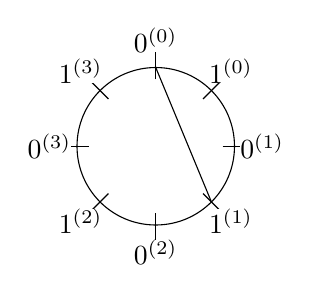
\begin{tikzpicture}
			\node [draw,circle,inner sep=0,minimum height=2cm] at (0,0) {};
			\foreach\y in {0,1,2,3} {
				\foreach\x in {0,1} {
					\draw[thin] (90-45*\x-90*\y:0.85) -- (90-45*\x-90*\y:1.35) node[fill=white,inner sep=0pt] {\x$^{(\y)}$};
				}
			}
			\draw (90:1) -- (-45:1);
			\end{tikzpicture}
%		\end{figure}
		
		Para escoger el segundo ciclo, su primera nota debe caer en el conjunto de v\'ertices m\'ultiplos de $d$ \textemdash de los que hay $\frac{n}{d}$. En el ejemplo ser\'ian los 0$^{(*)}$. Sin embargo, no podr\'ia ser cualquier m\'ultiplo, ya que si se escoge uno con posici\'on no coprima, el pol\'igono se cerrar\'ia antes de tiempo sin pasar por todos los v\'ertices. Entonces hay que escoger entre los v\'ertices coprimos, de los que hay $\varphi\left(\frac{n}{d}\right)$. Tras esto el pol\'igono est\'a totalmente determinado, y se puede formar de $\sum\limits_{d|n}\left(\varphi^2(\frac{n}{d})\cdot\left(\frac{n}{d}\right)^d\cdot d!\right)$ maneras.
		
		En nuestro ejemplo, si escogemos el siguiente comienzo del ciclo como el 0$^{(2)}$, como 2 no es coprimo con $\frac{n}{d}=4$, quedar\'ia de esta manera:
		
		\begin{multicols}{2}
			
			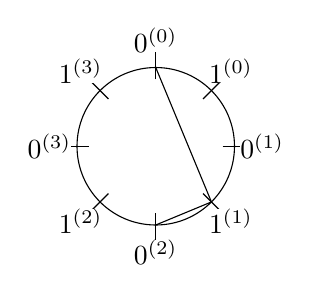
\begin{tikzpicture}
			\node [draw,circle,inner sep=0,minimum height=2cm] at (0,0) {};
			\foreach\y in {0,1,2,3} {
				\foreach\x in {0,1} {
					\draw[thin] (90-45*\x-90*\y:0.85) -- (90-45*\x-90*\y:1.35) node[fill=white,inner sep=0pt] {\x$^{(\y)}$};
				}
			}
			\draw (90:1) -- (-45:1) -- (-90:1);
			\end{tikzpicture}
			
			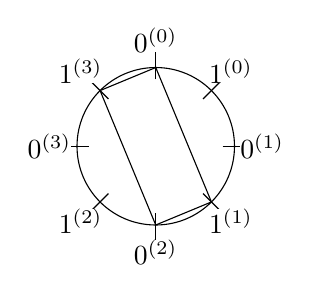
\begin{tikzpicture}
			\node [draw,circle,inner sep=0,minimum height=2cm] at (0,0) {};
			\foreach\y in {0,1,2,3} {
				\foreach\x in {0,1} {
					\draw[thin] (90-45*\x-90*\y:0.85) -- (90-45*\x-90*\y:1.35) node[fill=white,inner sep=0pt] {\x$^{(\y)}$};
				}
			}
			\draw (90:1) -- (-45:1) -- (-90:1);
			\draw[rotate=-180] (90:1) -- (-45:1) -- (-90:1);
			\end{tikzpicture}
	\end{multicols}
		Efectivamente, el diagrama se cierra antes de pasar por todos los v\'ertices. En cambio, si escogemos 0$^{(1)}$:
		\begin{multicols}{4}			
			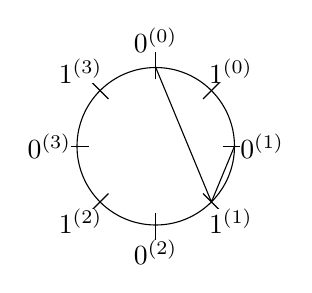
\begin{tikzpicture}
			\node [draw,circle,inner sep=0,minimum height=2cm] at (0,0) {};
			\foreach\y in {0,1,2,3} {
				\foreach\x in {0,1} {
					\draw[thin] (90-45*\x-90*\y:0.85) -- (90-45*\x-90*\y:1.35) node[fill=white,inner sep=0pt] {\x$^{(\y)}$};
				}
			}
		\draw (90:1) -- (-45:1) -- (0:1);
%		\draw[rotate=-90] (90:1) -- (-45:1) -- (0:1);
%		\draw[rotate=180] (90:1) -- (-45:1) -- (0:1);
%		\draw[rotate=90] (90:1) -- (-45:1) -- (0:1);
			\end{tikzpicture}
			
			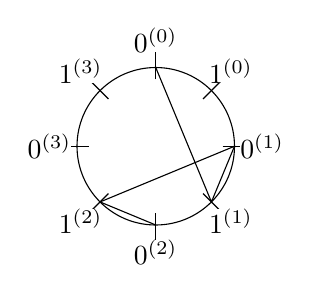
\begin{tikzpicture}
			\node [draw,circle,inner sep=0,minimum height=2cm] at (0,0) {};
			\foreach\y in {0,1,2,3} {
				\foreach\x in {0,1} {
					\draw[thin] (90-45*\x-90*\y:0.85) -- (90-45*\x-90*\y:1.35) node[fill=white,inner sep=0pt] {\x$^{(\y)}$};
				}
			}
			\draw (90:1) -- (-45:1) -- (0:1);
			\draw[rotate=-90] (90:1) -- (-45:1) -- (0:1);
%			\draw[rotate=180] (90:1) -- (-45:1) -- (0:1);
%			\draw[rotate=90] (90:1) -- (-45:1) -- (0:1);
			\end{tikzpicture}
			
			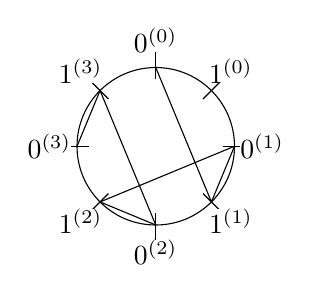
\begin{tikzpicture}
			\node [draw,circle,inner sep=0,minimum height=2cm] at (0,0) {};
			\foreach\y in {0,1,2,3} {
				\foreach\x in {0,1} {
					\draw[thin] (90-45*\x-90*\y:0.85) -- (90-45*\x-90*\y:1.35) node[fill=white,inner sep=0pt] {\x$^{(\y)}$};
				}
			}
			\draw (90:1) -- (-45:1) -- (0:1);
			\draw[rotate=-90] (90:1) -- (-45:1) -- (0:1);
			\draw[rotate=180] (90:1) -- (-45:1) -- (0:1);
%			\draw[rotate=90] (90:1) -- (-45:1) -- (0:1);
			\end{tikzpicture}
			
			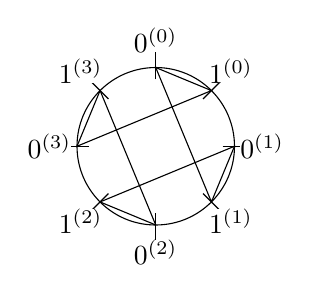
\begin{tikzpicture}
			\node [draw,circle,inner sep=0,minimum height=2cm] at (0,0) {};
			\foreach\y in {0,1,2,3} {
				\foreach\x in {0,1} {
					\draw[thin] (90-45*\x-90*\y:0.85) -- (90-45*\x-90*\y:1.35) node[fill=white,inner sep=0pt] {\x$^{(\y)}$};
				}
			}
			\draw (90:1) -- (-45:1) -- (0:1);
			\draw[rotate=-90] (90:1) -- (-45:1) -- (0:1);
			\draw[rotate=180] (90:1) -- (-45:1) -- (0:1);
			\draw[rotate=90] (90:1) -- (-45:1) -- (0:1);
			\end{tikzpicture}
		\end{multicols}
	
		Y con 0$^{(3)}$:
		\begin{multicols}{4}			
			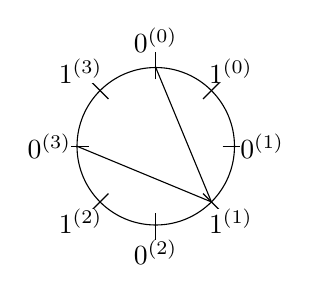
\begin{tikzpicture}
			\node [draw,circle,inner sep=0,minimum height=2cm] at (0,0) {};
			\foreach\y in {0,1,2,3} {
				\foreach\x in {0,1} {
					\draw[thin] (90-45*\x-90*\y:0.85) -- (90-45*\x-90*\y:1.35) node[fill=white,inner sep=0pt] {\x$^{(\y)}$};
				}
			}
			\draw (90:1) -- (-45:1) -- (180:1);
	%		\draw[rotate=-90] (90:1) -- (-45:1) -- (180:1);
	%		\draw[rotate=180] (90:1) -- (-45:1) -- (180:1);
	%		\draw[rotate=90] (90:1) -- (-45:1) -- (180:1);
			\end{tikzpicture}
			
			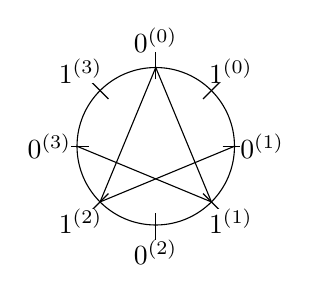
\begin{tikzpicture}
			\node [draw,circle,inner sep=0,minimum height=2cm] at (0,0) {};
			\foreach\y in {0,1,2,3} {
				\foreach\x in {0,1} {
					\draw[thin] (90-45*\x-90*\y:0.85) -- (90-45*\x-90*\y:1.35) node[fill=white,inner sep=0pt] {\x$^{(\y)}$};
				}
			}
			\draw (90:1) -- (-45:1) -- (180:1);
			\draw[rotate=-90] (90:1) -- (-45:1) -- (180:1);
	%		\draw[rotate=180] (90:1) -- (-45:1) -- (180:1);
	%		\draw[rotate=90] (90:1) -- (-45:1) -- (180:1);
			\end{tikzpicture}
			
			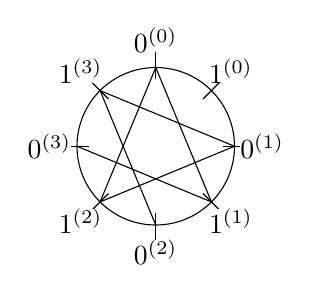
\begin{tikzpicture}
			\node [draw,circle,inner sep=0,minimum height=2cm] at (0,0) {};
			\foreach\y in {0,1,2,3} {
				\foreach\x in {0,1} {
					\draw[thin] (90-45*\x-90*\y:0.85) -- (90-45*\x-90*\y:1.35) node[fill=white,inner sep=0pt] {\x$^{(\y)}$};
				}
			}
			\draw (90:1) -- (-45:1) -- (180:1);
			\draw[rotate=-90] (90:1) -- (-45:1) -- (180:1);
			\draw[rotate=180] (90:1) -- (-45:1) -- (180:1);
	%		\draw[rotate=90] (90:1) -- (-45:1) -- (180:1);
			\end{tikzpicture}
			
			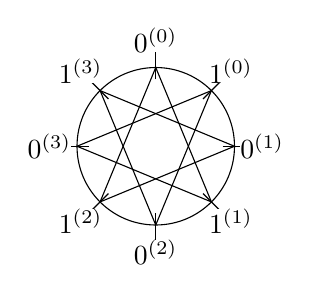
\begin{tikzpicture}
			\node [draw,circle,inner sep=0,minimum height=2cm] at (0,0) {};
			\foreach\y in {0,1,2,3} {
				\foreach\x in {0,1} {
					\draw[thin] (90-45*\x-90*\y:0.85) -- (90-45*\x-90*\y:1.35) node[fill=white,inner sep=0pt] {\x$^{(\y)}$};
				}
			}
			\draw (90:1) -- (-45:1) -- (180:1);
			\draw[rotate=-90] (90:1) -- (-45:1) -- (180:1);
			\draw[rotate=180] (90:1) -- (-45:1) -- (180:1);
			\draw[rotate=90] (90:1) -- (-45:1) -- (180:1);
			\end{tikzpicture}
		\end{multicols}
		
		Sea $d=3$ y $n=6$. Escogiendo el primer n\'umero como 0$^{(0)}$, el segundo como 1$^{(0)}$ y el tercero como 2$^{(1)}$, no queda m\'as remedio que escoger como comienzo del segundo ciclo el 0$^{(1)}$.
		
	\begin{multicols}{3}
		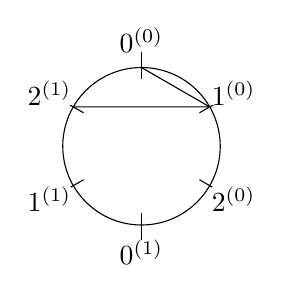
\begin{tikzpicture}
		\node [draw,circle,inner sep=0,minimum height=2cm] at (0,0) {};
		\foreach\y in {0,1} {
			\foreach\x in {0,1,2} {
				\draw[thin] (90-60*\x-180*\y:0.85) -- (90-60*\x-180*\y:1.35) node[fill=white,inner sep=0pt] {\x$^{(\y)}$};
			}
		}
		\draw (90:1) -- (30:1) -- (150:1);
		\end{tikzpicture}
		
		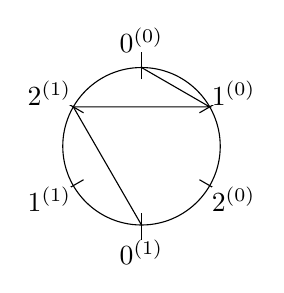
\begin{tikzpicture}
		\node [draw,circle,inner sep=0,minimum height=2cm] at (0,0) {};
		\foreach\y in {0,1} {
			\foreach\x in {0,1,2} {
				\draw[thin] (90-60*\x-180*\y:0.85) -- (90-60*\x-180*\y:1.35) node[fill=white,inner sep=0pt] {\x$^{(\y)}$};
			}
		}
		\draw (90:1) -- (30:1) -- (150:1) -- (-90:1);
		%		\draw[rotate=180] (90:1) -- (30:1) -- (150:1) -- (-90:1);
		\end{tikzpicture}
		
		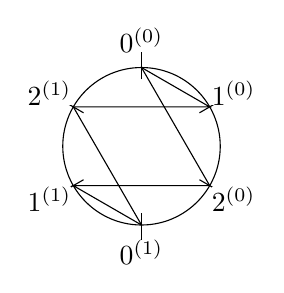
\begin{tikzpicture}
		\node [draw,circle,inner sep=0,minimum height=2cm] at (0,0) {};
		\foreach\y in {0,1} {
			\foreach\x in {0,1,2} {
				\draw[thin] (90-60*\x-180*\y:0.85) -- (90-60*\x-180*\y:1.35) node[fill=white,inner sep=0pt] {\x$^{(\y)}$};
			}
		}
		\draw (90:1) -- (30:1) -- (150:1) -- (-90:1);
		\draw[rotate=180] (90:1) -- (30:1) -- (150:1) -- (-90:1);
		\end{tikzpicture}
	\end{multicols}

		Pero tambi\'en podr\'ia aparecer este mismo comienzo con la parte final dada la vuelta, sim\'etrica, de esta manera: 0$^{(0)}$, 1$^{(0)}$, 2$^{(1)}$, 2$^{(0)}$, 1$^{(1)}$, 0$^{(1)}$. Esta construcci\'on no est\'a incluida en lo descrito anteriormente, y sin embargo es invariante con respecto a T, V y C a la vez. 
		
		\begin{multicols}{3}
			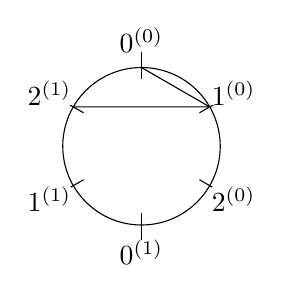
\begin{tikzpicture}
			\node [draw,circle,inner sep=0,minimum height=2cm] at (0,0) {};
			\foreach\y in {0,1} {
				\foreach\x in {0,1,2} {
					\draw[thin] (90-60*\x-180*\y:0.85) -- (90-60*\x-180*\y:1.35) node[fill=white,inner sep=0pt] {\x$^{(\y)}$};
				}
			}
			\draw (90:1) -- (30:1) -- (150:1);
			\end{tikzpicture}
			
			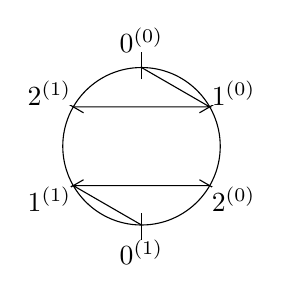
\begin{tikzpicture}
			\node [draw,circle,inner sep=0,minimum height=2cm] at (0,0) {};
			\foreach\y in {0,1} {
				\foreach\x in {0,1,2} {
					\draw[thin] (90-60*\x-180*\y:0.85) -- (90-60*\x-180*\y:1.35) node[fill=white,inner sep=0pt] {\x$^{(\y)}$};
				}
			}
			\draw (90:1) -- (30:1) -- (150:1);
			\draw[rotate=180] (90:1) -- (30:1) -- (150:1);
			\end{tikzpicture}
			
			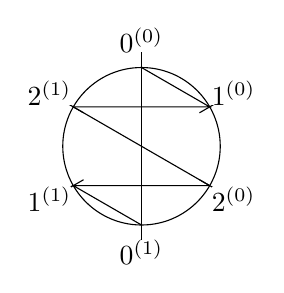
\begin{tikzpicture}
			\node [draw,circle,inner sep=0,minimum height=2cm] at (0,0) {};
			\foreach\y in {0,1} {
				\foreach\x in {0,1,2} {
					\draw[thin] (90-60*\x-180*\y:0.85) -- (90-60*\x-180*\y:1.35) node[fill=white,inner sep=0pt] {\x$^{(\y)}$};
				}
			}
			\draw (90:1) -- (30:1) -- (150:1);
			\draw[rotate=180] (90:1) -- (30:1) -- (150:1);
			\draw[] (-90:1) -- (90:1);
			\draw[] (150:1) -- (-30:1);
			\end{tikzpicture}
		\end{multicols}
		
		Y es que con $n$ par, al rotar $\uptheta_{{n}/{2}}$ el diagrama, \'este puede llegar con la orientaci\'on cambiada. Esto puede ocurrir cuando haya una diagonal; es decir, cuando entre dos notas haya un intervalo de $\frac{n}{2}$.
		
		\begin{center}
		\begin{tikzpicture}[ddiagram]
		\ddiagram[no tikz]{0,1,5,2,4,3}
		
		\draw[style=ddihedralArrow] (2.5,0) -- node[above=5pt] {T$^3$} (4,0);
		
		\ddiagram[no tikz, xshift=4cm]{3,4,2,5,1,0}
		
		\draw[style=ddihedralArrow,xshift=6cm] (2.5,0) -- node[above=5pt] {V} (4,0);
		
		\ddiagram[no tikz, xshift=8cm, arrow shift=1.25]{3,0,1,5,2,4}
		
		\draw[style=ddihedralArrow] (12.3,-2.5) -- (12.3,-3.25) -- node [fill=white] {C} (0,-3.25) -- (0,-2.5);
		\end{tikzpicture}
		\end{center}
		
		Se escoge el primer punto de entre $\frac{n}{2}$ posibilidades. No son $n$ ya que saldr\'ia la misma figura si se escoge el punto antipodal.
		Con una rotaci\'on de $\uptheta_{{n}/{2}}$, el primer ciclo se escoge igual que antes, de $\left(\frac{n}{n/2}\right)^{\frac{n}{2}}\cdot \frac{n}{2}!=2^{\frac{n}{2}}\cdot \frac{n}{2}!$ maneras. Y con esto ya queda la figura determinada. Esto lleva a las $\frac{n}{2}\cdot2^{\frac{n}{2}}\cdot\frac{n}{2}!$ formas de dibujar un pol\'igono con las caracter\'isticas buscadas.
		
		\subsubsection[Elementos estables mediante $S$]{Elementos estables mediante $\bm{S}$}
		
		Los elementos estables mediante $S$ son aquellos que quedan invariantes mediante reflexiones. En este punto se ha de separar por paridad de $n$. 
		
		Para $n$ impar, existen $n$ reflexiones para cada uno de los ejes de simetr\'ia que pasan por cada v\'ertice. Despu\'es, hay $n$ formas de escoger el primer v\'ertice de la secuencia. Ahora hay $\frac{n-1}{2}$ parejas de v\'ertices; se escoge los primeros miembros entre ellos de $2^{\frac{n-1}{2}}$ formas, tras lo cual \'estos se ordenan de $\frac{n-1}{2}!$ formas. Esto da un resultado de  $n^2\cdot2^{\frac{n-1}{2}}\cdot\frac{n-1}{2}!$ pol\'igonos invariantes.
		
		Para $n$ par se tienen dos simetr\'ias: con ejes que pasan por v\'ertices y con ejes que pasan por lados. De manera similar a la anterior, se escoge el eje, el primer v\'ertice, los primeros miembros de las parejas de v\'ertices y se ordenan. Para las simetr\'ias con ejes que pasan por v\'ertices, da un resultado de  $\frac{n^2}{2}\cdot2^{\frac{n}{2}}\cdot\left(\frac{n}{2}-1\right)!$. Para las simetr\'ias con ejes que pasan por lados, da un resultado de $\frac{n^2}{2}\cdot2^{\frac{n}{2}-1}\cdot\frac{n}{2}!$.
		
		\subsubsection*{Suma completa}
		
		En resumen, estos a continuaci\'on son los numeradores $\sum%_{\Psi\in\mbox{D}_{n}\times\mbox{D}_{n}}
		{Fij}(\Psi)$. El resultado final del n\'umero de diagramas posibles, o espectros seriales distintos, es dicho numerador entre $4n^2$, el tama\~no del grupo. 	
		\def\arraystretch{1.5}
		\[\begin{array}{c||c}
		&\textbf{\textit{n} IMPAR}\\\hline\hline
		\mbox{Rotaci\'on}&\sum\limits_{d|n}\left(\varphi^2(\frac{n}{d})\cdot\left(\frac{n}{d}\right)^d\cdot d!\right)\\\hline
		\mbox{Reflexi\'on}&n^2\cdot2^{\frac{n-1}{2}}\cdot\frac{n-1}{2}!\\\hline
		&\sum\limits_{d|n}\left(\varphi^2(\frac{n}{d})\cdot\left(\frac{n}{d}\right)^d\cdot d!\right)+n^2\cdot2^{\frac{n-1}{2}}\cdot\frac{n-1}{2}!\\
		\end{array}\]
		
		\[\begin{array}{c||c}
		&\textbf{\textit{n} PAR}\\\hline\hline
		\mbox{Rotaci\'on I}&\sum\limits_{d|n}\left(\varphi^2(\frac{n}{d})\cdot\left(\frac{n}{d}\right)^d\cdot d!\right)\\\hline
		\mbox{Rotaci\'on II}&\frac{n}{2}\cdot2^{\frac{n}{2}}\cdot\frac{n}{2}!\\\hline
		\mbox{Reflexi\'on v\'ertices}&\frac{n^2}{2}\cdot2^{\frac{n}{2}}\cdot\left(\frac{n}{2}-1\right)!\\\hline
		\mbox{Reflexi\'on lados}&\frac{n^2}{2}\cdot2^{\frac{n}{2}-1}\cdot\frac{n}{2}!\\\hline
		&\sum\limits_{d|n}\left(\varphi^2(\frac{n}{d})\cdot\left(\frac{n}{d}\right)^d\cdot d!\right)+\frac{n(n+6)}{4}\cdot2^{\frac{n}{2}}\cdot\frac{n}{2}!\\
		\end{array}\]
		\def\arraystretch{1}
		
	\subsection{Medefonismo, monofonismo y difonismo}
	\label{monodi}
		Con $n=0$ se da el caso de medefonismo. El grupo sim\'etrico de orden 0 tiene $0!=1$ elemento. Por tanto, hay una sola posible serie, $\sigma$, que es la que no tiene ninguna nota. El medefonismo es com\'unmente llamado silencio.
		
		\[\sigma=\drow{}
		\qquad\qquad\qquad
		\begin{array}{l||r}
		&\\
		\hline
		\hline
		&\\
		\hline
		&
		\end{array}\]
	
		Con $n=1$ se da el caso de monofonismo. Con solamente una posible nota, el grupo sim\'etrico de orden 1 tiene $1!=1$ elemento. Por tanto, hay una sola posible serie, $\sigma_0$, que es igual a su inversa, a su retrogradaci\'on y a su retrogradaci\'on inversa:
		\[\sigma_0=\drow{0}
		\qquad\qquad\qquad
		\begin{array}{l|c|r}
			&{I}_{0}&\\
			\hline
			{T}_{0}&0&{R}_{0}\\
			\hline
			&{IR}_{0}&\\
			\hline
			&{RI}_{0}&
		\end{array}\]
	
		Con $n=2$ se da el caso de difonismo. Tiene dos posibles notas, as\'i que su grupo sim\'etrico, el de orden 2, tiene $2!=2$ elementos. Por tanto, hay dos series distintas, $\sigma_0$ y $\sigma_1$. Se puede observar que ambas pertenecen al mismo espectro serial, dado que $\sigma_1={T}^1(\sigma_0)$. Adem\'as, al igual que en el monofonismo, ambas coinciden con sus inversas, incumpliendo la regla general para $n>2$ probada en el apartado \ref{inversano}.
		\[\sigma_0=\drow{0,1}
		\qquad\qquad
		\begin{array}{l|cc|r}
			&{I}_{0}&{I}_{1}&\\
			\hline
			{T}_{0}&0&1&{R}_{0}\\
			{T}_{1}&1&0&{R}_{1}\\
			\hline
			&{IR}_{0}&{IR}_{1}&\\
			\hline
			&{RI}_{0}&{RI}_{1}&
		\end{array}
		\qquad\qquad
		\sigma_1=\drow{1,0}\]